\subsection*{Problema 43}

\textbf{Enunciado:} \\
Calcular la integral indefinida:
\begin{align*}
\int x^3 (1 - x^2)^{-3/2} \, dx
\end{align*}

\textbf{Solución:} \\
Para resolver esta integral, utilizaremos el método de sustitución algebraica. 
Definimos la nueva variable $u$ y su respectiva derivada de la siguiente manera:
\begin{align*}
u &= 1 - x^2 \\
du &= -2x \, dx \implies x \, dx = -\dfrac{1}{2} \, du
\end{align*}

De la definición de $u$, podemos expresar $x^2$ en términos de $u$:
\begin{align*}
x^2 = 1 - u
\end{align*}

Reescribimos la integral original separando un término $x$ para construir la expresión $x \, dx$:
\begin{align*}
\int x^2 \cdot (1 - x^2)^{-3/2} \cdot (x \, dx)
\end{align*}

Sustituimos $x^2$, $1 - x^2$ y $x \, dx$ en la integral:
\begin{align*}
\int (1 - u) \cdot (u)^{-3/2} \cdot \left(-\dfrac{1}{2} \, du\right)
\end{align*}

Sacamos la constante fuera de la integral y distribuimos el término $u^{-3/2}$:
\begin{align*}
-\dfrac{1}{2} \int (u^{-3/2} - u^{-1/2}) \, du
\end{align*}

Integramos término a término usando la regla de la potencia:
\begin{align*}
&= -\dfrac{1}{2} \left[ \dfrac{u^{-1/2}}{-1/2} - \dfrac{u^{1/2}}{1/2} \right] \\
&= -\dfrac{1}{2} \left[ -2u^{-1/2} - 2u^{1/2} \right]
\end{align*}

Simplificamos el factor escalar $-\dfrac{1}{2}$ con el paréntesis:
\begin{align*}
&= u^{-1/2} + u^{1/2} + C \\
&= \dfrac{1}{\sqrt{u}} + \sqrt{u} + C
\end{align*}

Finalmente, regresamos a la variable original $x$ sustituyendo $u = 1 - x^2$:
\begin{align*}
&= \dfrac{1}{\sqrt{1 - x^2}} + \sqrt{1 - x^2} + C
\end{align*}

Podemos expresar el resultado bajo un mismo denominador común:
\begin{align*}
&= \dfrac{1 + (1 - x^2)}{\sqrt{1 - x^2}} + C \\
&= \dfrac{2 - x^2}{\sqrt{1 - x^2}} + C
\end{align*}

\begin{figure}[H]
	\centering
	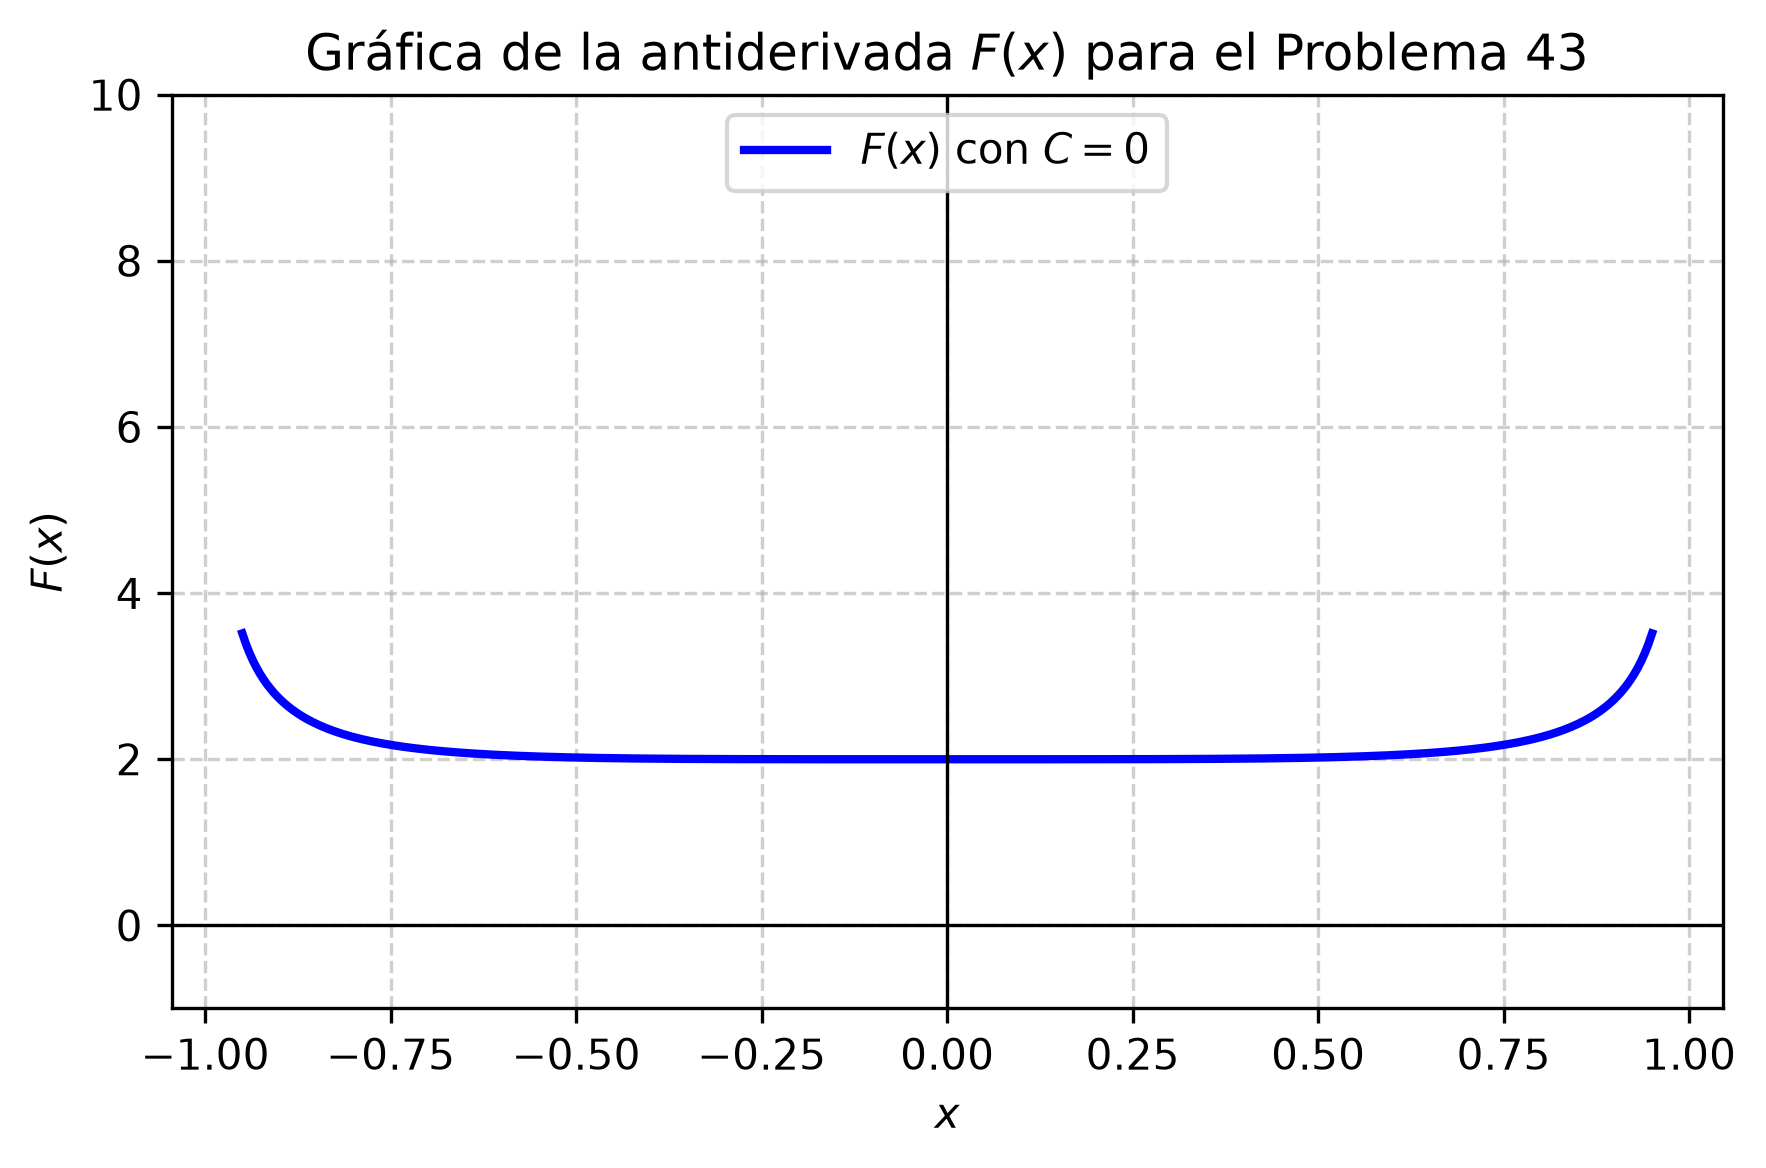
\includegraphics[width=\columnwidth]{semana_05/graficas/SEM05_P43_grafica.png}
	\caption{Representación gráfica de $f(x)$ y su antiderivada $F(x)$ evaluada para la constante de integración $C = 0$ (Problema 43).}
	\label{fig:problema43}
\end{figure}
